\section{Cenário de Teste 1}

Este cenário está dividido em 5 (cinco) exemplos, os quais são apresentados a seguir, contemplando todo o processo de auto-localização
em cada exemplo, a partir da apresentação das Imagens abaixo.

\subsection{Exemplo 1}

Exemplo utilizando 200 partículas:

\begin{figure}[H]
  \centering
  \includegraphics[scale=1]{figuras/cen1_ex1/1.eps}
  \caption[Partículas Iniciais]{Partículas iniciais}
  \label{img:cen1_ex1_1}
\end{figure}

\begin{figure}[H]
  \centering
  \includegraphics[scale=1]{figuras/cen1_ex1/2.eps}
  \caption[Primeiro Ciclo de Filtragem]{Primeiro ciclo de filtragem}
  \label{img:cen1_ex1_2}
\end{figure}

\begin{figure}[H]
  \centering
  \includegraphics[scale=1]{figuras/cen1_ex1/3.eps}
  \caption[Segundo Ciclo de Filtragem]{Segundo ciclo de filtragem}
  \label{img:cen1_ex1_3}
\end{figure}

\begin{figure}[H]
  \centering
  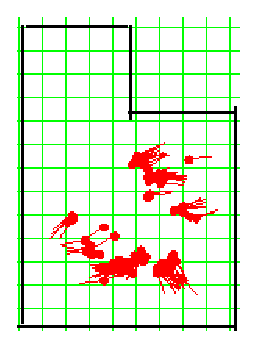
\includegraphics[scale=1]{figuras/cen1_ex1/4.eps}
  \caption[Terceiro Ciclo de Filtragem]{Terceiro ciclo de filtragem}
  \label{img:cen1_ex1_4}
\end{figure}

\begin{figure}[H]
  \centering
  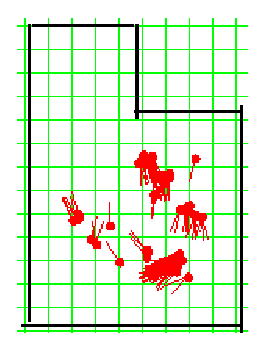
\includegraphics[scale=1]{figuras/cen1_ex1/5.eps}
  \caption[Quarto Ciclo de Filtragem]{Quarto ciclo de filtragem}
  \label{img:cen1_ex1_5}
\end{figure}

\begin{figure}[H]
  \centering
  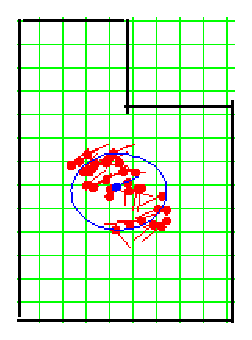
\includegraphics[scale=1]{figuras/cen1_ex1/6.eps}
  \caption[Quinto Ciclo de Filtragem]{Quinto ciclo de filtragem}
  \label{img:cen1_ex1_6}
\end{figure}

\begin{figure}[H]
  \centering
  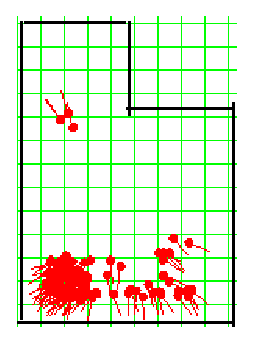
\includegraphics[scale=1]{figuras/cen1_ex1/7.eps}
  \caption[Sexto Ciclo de Filtragem]{Sexto ciclo de filtragem}
  \label{img:cen1_ex1_7}
\end{figure}

\begin{figure}[H]
  \centering
  \includegraphics[scale=1]{figuras/cen1_ex1/8.eps}
  \caption[Sétimo Ciclo de Filtragem]{Sétimo ciclo de filtragem}
  \label{img:cen1_ex1_8}
\end{figure}

\begin{figure}[H]
  \centering
  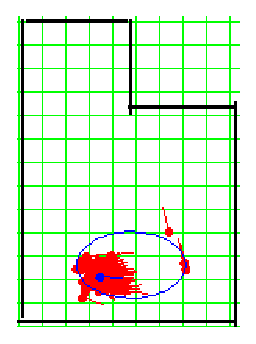
\includegraphics[scale=1]{figuras/cen1_ex1/9.eps}
  \caption[Oitavo Ciclo de Filtragem]{Oitavo ciclo de filtragem}
  \label{img:cen1_ex1_9}
\end{figure}

\begin{figure}[H]
  \centering
  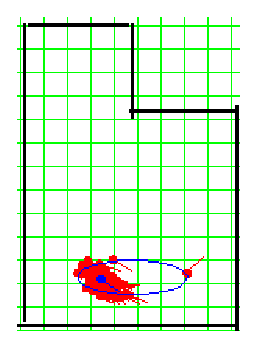
\includegraphics[scale=1]{figuras/cen1_ex1/10.eps}
  \caption[Nono Ciclo de Filtragem]{Nono ciclo de filtragem}
  \label{img:cen1_ex1_10}
\end{figure}

\subsection{Exemplo 2}

Exemplo utilizando 400 partículas:

\begin{figure}[H]
  \centering
  \includegraphics[scale=1]{figuras/cen1_ex2/1.eps}
  \caption[Partículas Iniciais]{Partículas iniciais}
  \label{img:cen1_ex2_1}
\end{figure}

\begin{figure}[H]
  \centering
  \includegraphics[scale=1]{figuras/cen1_ex2/2.eps}
  \caption[Primeiro Ciclo de Filtragem]{Primeiro ciclo de filtragem}
  \label{img:cen1_ex2_2}
\end{figure}

\begin{figure}[H]
  \centering
  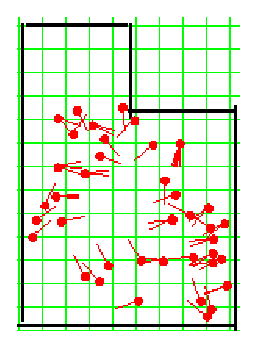
\includegraphics[scale=1]{figuras/cen1_ex2/3.eps}
  \caption[Segundo Ciclo de Filtragem]{Segundo ciclo de filtragem}
  \label{img:cen1_ex2_3}
\end{figure}

\begin{figure}[H]
  \centering
  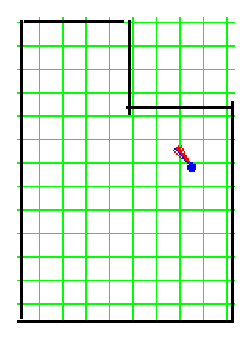
\includegraphics[scale=1]{figuras/cen1_ex2/4.eps}
  \caption[Terceiro Ciclo de Filtragem]{Terceiro ciclo de filtragem}
  \label{img:cen1_ex2_4}
\end{figure}

\begin{figure}[H]
  \centering
  \includegraphics[scale=1]{figuras/cen1_ex2/5.eps}
  \caption[Quarto Ciclo de Filtragem]{Quarto ciclo de filtragem}
  \label{img:cen1_ex2_5}
\end{figure}

\begin{figure}[H]
  \centering
  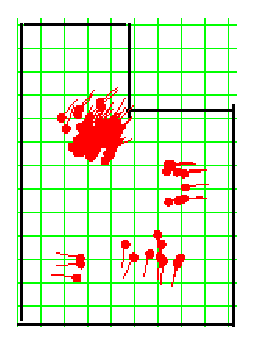
\includegraphics[scale=1]{figuras/cen1_ex2/6.eps}
  \caption[Quinto Ciclo de Filtragem]{Quinto ciclo de filtragem}
  \label{img:cen1_ex2_6}
\end{figure}

\begin{figure}[H]
  \centering
  \includegraphics[scale=1]{figuras/cen1_ex2/7.eps}
  \caption[Sexto Ciclo de Filtragem]{Sexto ciclo de filtragem}
  \label{img:cen1_ex2_7}
\end{figure}

\begin{figure}[H]
  \centering
  \includegraphics[scale=1]{figuras/cen1_ex2/8.eps}
  \caption[Sétimo Ciclo de Filtragem]{Sétimo ciclo de filtragem}
  \label{img:cen1_ex2_8}
\end{figure}

\begin{figure}[H]
  \centering
  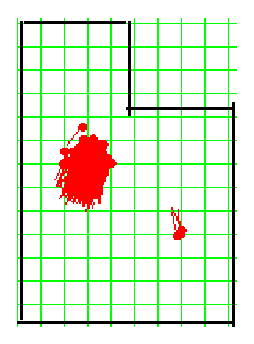
\includegraphics[scale=1]{figuras/cen1_ex2/9.eps}
  \caption[Oitavo Ciclo de Filtragem]{Oitavo ciclo de filtragem}
  \label{img:cen1_ex2_9}
\end{figure}

\begin{figure}[H]
  \centering
  \includegraphics[scale=1]{figuras/cen1_ex2/10.eps}
  \caption[Nono Ciclo de Filtragem]{Nono ciclo de filtragem}
  \label{img:cen1_ex2_10}
\end{figure}

\begin{figure}[H]
  \centering
  \includegraphics[scale=1]{figuras/cen1_ex2/11.eps}
  \caption[Décimo Ciclo de Filtragem]{Décimo ciclo de filtragem}
  \label{img:cen1_ex2_11}
\end{figure}

\subsection{Exemplo 3}

Exemplo utilizando 500 partículas:

\begin{figure}[H]
  \centering
  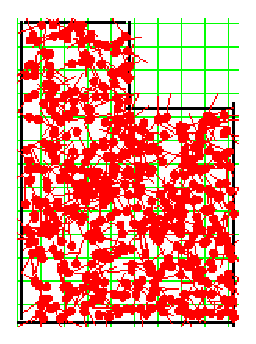
\includegraphics[scale=1]{figuras/cen1_ex3/1.eps}
  \caption[Partículas Iniciais]{Partículas iniciais}
  \label{img:cen1_ex3_1}
\end{figure}

\begin{figure}[H]
  \centering
  \includegraphics[scale=1]{figuras/cen1_ex3/2.eps}
  \caption[Primeiro Ciclo de Filtragem]{Primeiro ciclo de filtragem}
  \label{img:cen1_ex3_2}
\end{figure}

\begin{figure}[H]
  \centering
  \includegraphics[scale=1]{figuras/cen1_ex3/3.eps}
  \caption[Segundo Ciclo de Filtragem]{Segundo ciclo de filtragem}
  \label{img:cen1_ex3_3}
\end{figure}

\begin{figure}[H]
  \centering
  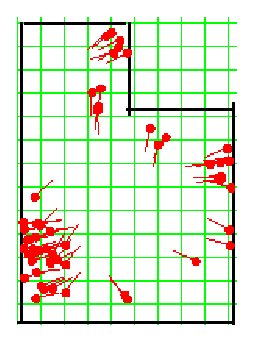
\includegraphics[scale=1]{figuras/cen1_ex3/4.eps}
  \caption[Terceiro Ciclo de Filtragem]{Terceiro ciclo de filtragem}
  \label{img:cen1_ex3_4}
\end{figure}

\begin{figure}[H]
  \centering
  \includegraphics[scale=1]{figuras/cen1_ex3/5.eps}
  \caption[Quarto Ciclo de Filtragem]{Quarto ciclo de filtragem}
  \label{img:cen1_ex3_5}
\end{figure}

\begin{figure}[H]
  \centering
  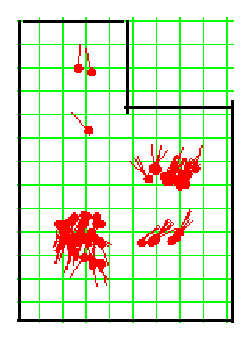
\includegraphics[scale=1]{figuras/cen1_ex3/6.eps}
  \caption[Quinto Ciclo de Filtragem]{Quinto ciclo de filtragem}
  \label{img:cen1_ex3_6}
\end{figure}

\begin{figure}[H]
  \centering
  \includegraphics[scale=1]{figuras/cen1_ex3/7.eps}
  \caption[Sexto Ciclo de Filtragem]{Sexto ciclo de filtragem}
  \label{img:cen1_ex3_7}
\end{figure}

\begin{figure}[H]
  \centering
  \includegraphics[scale=1]{figuras/cen1_ex3/8.eps}
  \caption[Sétimo Ciclo de Filtragem]{Sétimo ciclo de filtragem}
  \label{img:cen1_ex3_8}
\end{figure}

\begin{figure}[H]
  \centering
  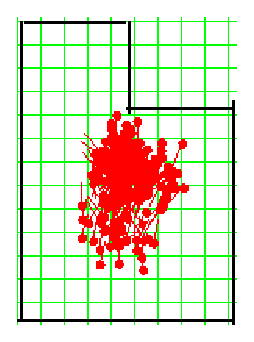
\includegraphics[scale=1]{figuras/cen1_ex3/9.eps}
  \caption[Oitavo Ciclo de Filtragem]{Oitavo ciclo de filtragem}
  \label{img:cen1_ex3_9}
\end{figure}

\begin{figure}[H]
  \centering
  \includegraphics[scale=1]{figuras/cen1_ex3/10.eps}
  \caption[Nono Ciclo de Filtragem]{Nono ciclo de filtragem}
  \label{img:cen1_ex3_10}
\end{figure}

\begin{figure}[H]
  \centering
  \includegraphics[scale=1]{figuras/cen1_ex3/11.eps}
  \caption[Décimo Ciclo de Filtragem]{Décimo ciclo de filtragem}
  \label{img:cen1_ex3_11}
\end{figure}

\begin{figure}[H]
  \centering
  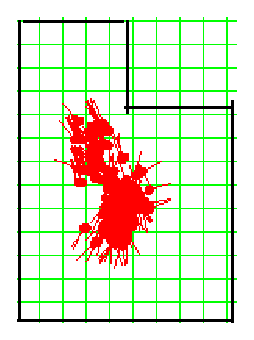
\includegraphics[scale=1]{figuras/cen1_ex3/12.eps}
  \caption[Décimo Primeiro Ciclo de Filtragem]{Décimo Primeiro ciclo de filtragem}
  \label{img:cen1_ex3_12}
\end{figure}

\begin{figure}[H]
  \centering
  \includegraphics[scale=1]{figuras/cen1_ex3/13.eps}
  \caption[Décimo Segundo Ciclo de Filtragem]{Décimo Segundo ciclo de filtragem}
  \label{img:cen1_ex3_13}
\end{figure}

\begin{figure}[H]
  \centering
  \includegraphics[scale=1]{figuras/cen1_ex3/14.eps}
  \caption[Décimo Terceiro Ciclo de Filtragem]{Décimo Terceiro ciclo de filtragem}
  \label{img:cen1_ex3_14}
\end{figure}

\begin{figure}[H]
  \centering
  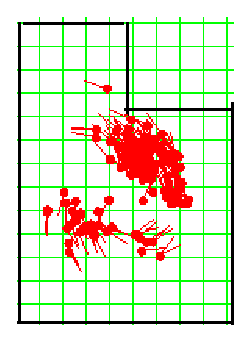
\includegraphics[scale=1]{figuras/cen1_ex3/15.eps}
  \caption[Décimo Quarto Ciclo de Filtragem]{Décimo Quarto ciclo de filtragem}
  \label{img:cen1_ex3_15}
\end{figure}

\begin{figure}[H]
  \centering
  \includegraphics[scale=1]{figuras/cen1_ex3/16.eps}
  \caption[Décimo Quinto Ciclo de Filtragem]{Décimo Quinto ciclo de filtragem}
  \label{img:cen1_ex3_16}
\end{figure}

\begin{figure}[H]
  \centering
  \includegraphics[scale=1]{figuras/cen1_ex3/17.eps}
  \caption[Décimo Sexto Ciclo de Filtragem]{Décimo Sexto ciclo de filtragem}
  \label{img:cen1_ex3_17}
\end{figure}

\begin{figure}[H]
  \centering
  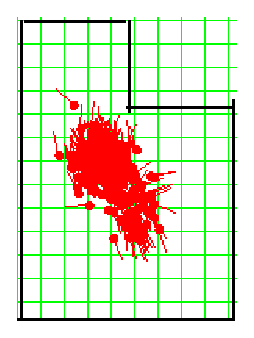
\includegraphics[scale=1]{figuras/cen1_ex3/18.eps}
  \caption[Décimo Sétimo Ciclo de Filtragem]{Décimo Sétimo ciclo de filtragem}
  \label{img:cen1_ex3_18}
\end{figure}

\begin{figure}[H]
  \centering
  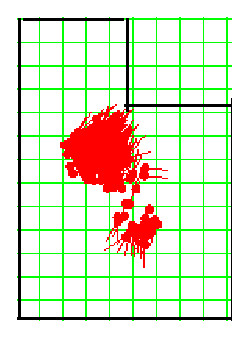
\includegraphics[scale=1]{figuras/cen1_ex3/19.eps}
  \caption[Décimo Oitavo Ciclo de Filtragem]{Décimo Oitavo ciclo de filtragem}
  \label{img:cen1_ex3_19}
\end{figure}

\begin{figure}[H]
  \centering
  \includegraphics[scale=1]{figuras/cen1_ex3/20.eps}
  \caption[Décimo Nono Ciclo de Filtragem]{Décimo Nono ciclo de filtragem}
  \label{img:cen1_ex3_20}
\end{figure}

\begin{figure}[H]
  \centering
  \includegraphics[scale=1]{figuras/cen1_ex3/21.eps}
  \caption[Vigésimo Ciclo de Filtragem]{Vigésimo ciclo de filtragem}
  \label{img:cen1_ex3_21}
\end{figure}

\begin{figure}[H]
  \centering
  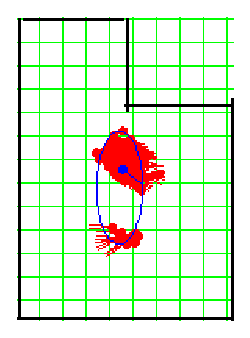
\includegraphics[scale=1]{figuras/cen1_ex3/22.eps}
  \caption[Vigésimo Primeiro Ciclo de Filtragem]{Vigésimo Primeiro ciclo de filtragem}
  \label{img:cen1_ex3_22}
\end{figure}

\begin{figure}[H]
  \centering
  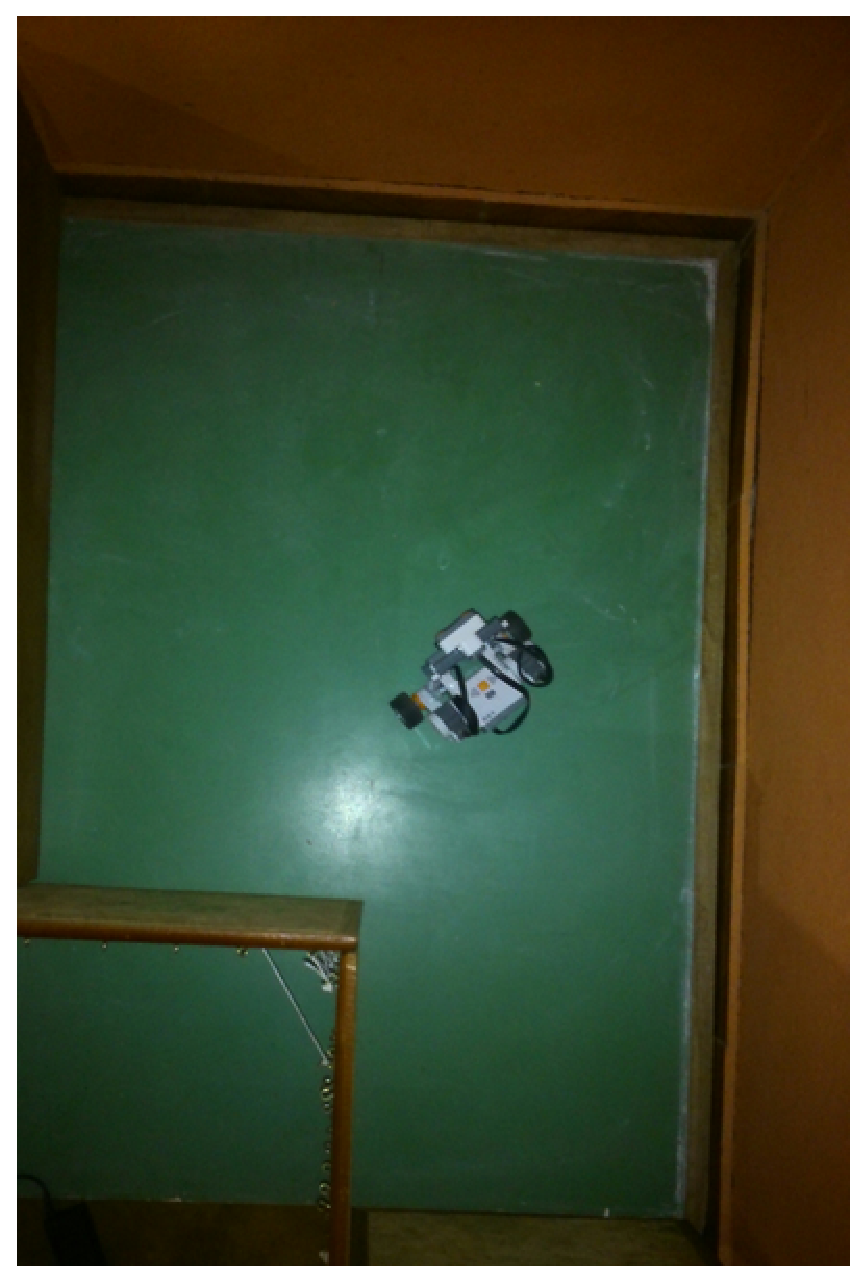
\includegraphics[scale=1]{figuras/cen1_ex3/real.eps}
  \caption[Posição Real do Robô]{Posição Real do Robô.}
  \label{img:cen1_ex3_23}
\end{figure}


\subsection{Exemplo 4}

Exemplo utilizando 100 partículas:

\begin{figure}[H]
  \centering
  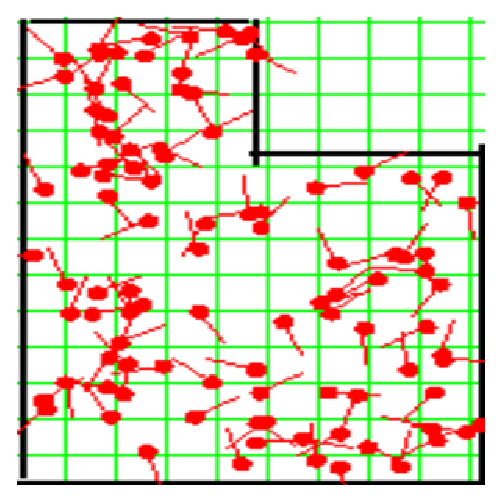
\includegraphics[scale=0.6]{figuras/cen1_ex4/1.eps}
  \caption[Partículas Iniciais]{Partículas iniciais}
  \label{img:cen1_ex4_1}
\end{figure}

\begin{figure}[H]
  \centering
  \includegraphics[scale=0.6]{figuras/cen1_ex4/2.eps}
  \caption[Primeiro Ciclo de Filtragem]{Primeiro ciclo de filtragem}
  \label{img:cen1_ex4_2}
\end{figure}

\begin{figure}[H]
  \centering
  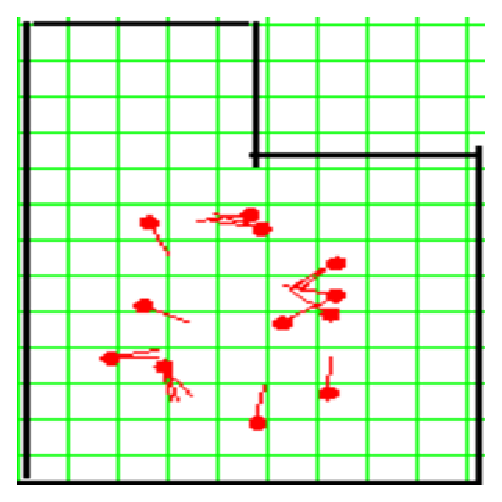
\includegraphics[scale=0.6]{figuras/cen1_ex4/3.eps}
  \caption[Segundo Ciclo de Filtragem]{Segundo ciclo de filtragem}
  \label{img:cen1_ex4_3}
\end{figure}

\begin{figure}[H]
  \centering
  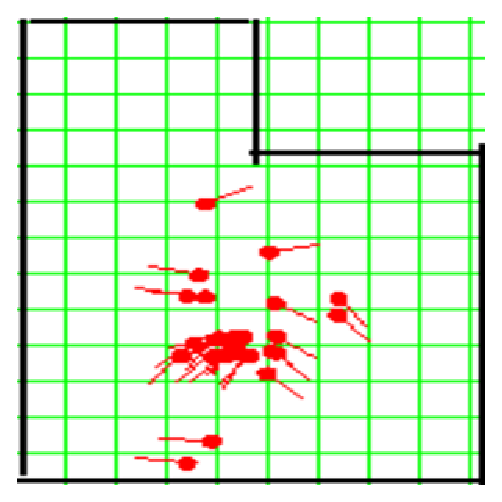
\includegraphics[scale=0.6]{figuras/cen1_ex4/4.eps}
  \caption[Terceiro Ciclo de Filtragem]{Terceiro ciclo de filtragem}
  \label{img:cen1_ex4_4}
\end{figure}

\begin{figure}[H]
  \centering
  \includegraphics[scale=0.6]{figuras/cen1_ex4/5.eps}
  \caption[Quarto Ciclo de Filtragem]{Quarto ciclo de filtragem}
  \label{img:cen1_ex4_5}
\end{figure}

\begin{figure}[H]
  \centering
  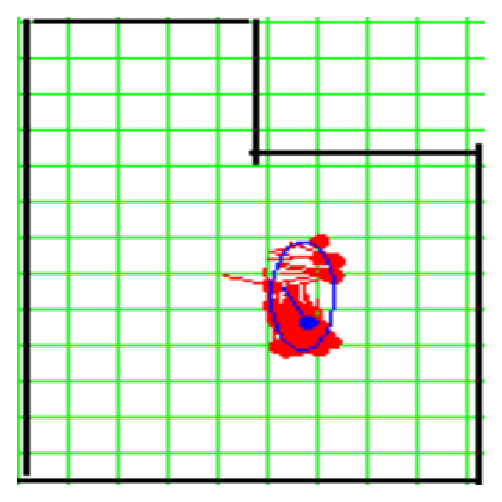
\includegraphics[scale=0.6]{figuras/cen1_ex4/6.eps}
  \caption[Quinto Ciclo de Filtragem]{Quinto ciclo de filtragem}
  \label{img:cen1_ex4_6}
\end{figure}

\begin{figure}[H]
  \centering
  \includegraphics[scale=0.8]{figuras/cen1_ex4/real.eps}
  \caption[Posição real do Robô]{Posição Real do Robô.}
  \label{img:cen1_ex4_6}
\end{figure}

\subsection{Exemplo 5}

Exemplo utilizando 150 partículas:

\begin{figure}[H]
  \centering
  \includegraphics[scale=1]{figuras/cen1_ex5/1.eps}
  \caption[Partículas Iniciais]{Partículas iniciais}
  \label{img:cen1_ex5_1}
\end{figure}

\begin{figure}[H]
  \centering
  \includegraphics[scale=1]{figuras/cen1_ex5/2.eps}
  \caption[Primeiro Ciclo de Filtragem]{Primeiro ciclo de filtragem}
  \label{img:cen1_ex5_2}
\end{figure}

\begin{figure}[H]
  \centering
  \includegraphics[scale=1]{figuras/cen1_ex5/3.eps}
  \caption[Segundo Ciclo de Filtragem]{Segundo ciclo de filtragem}
  \label{img:cen1_ex5_3}
\end{figure}

\begin{figure}[H]
  \centering
  \includegraphics[scale=1]{figuras/cen1_ex5/4.eps}
  \caption[Terceiro Ciclo de Filtragem]{Terceiro ciclo de filtragem}
  \label{img:cen1_ex5_4}
\end{figure}

\begin{figure}[H]
  \centering
  \includegraphics[scale=0.8]{figuras/cen1_ex5/real.eps}
  \caption[Posição real do Robô]{Posição Real do Robô.}
  \label{img:cen1_ex5_6}
\end{figure}
